%----------------------------------------------------------------------------------------

\documentclass[spanish]{article}
\usepackage[utf8]{inputenc} % Para poner acentos automáticamente y demas
\usepackage[spanish]{babel} % Para trabajar en español
%\usepackage[sc]{mathpazo} % Use the Palatino font


\usepackage[square,sort&compress]{natbib} % Use the natbib reference package - read up on this to edit the reference style; if you want text (e.g. Smith et al., 2012) for the in-text references (instead of numbers), remove 'numbers' 
\usepackage{graphicx} % para incluir imagenes
\usepackage{caption}
\usepackage{subcaption}
\usepackage{wrapfig}
\usepackage{titling}
\usepackage[T1]{fontenc} % Use 8-bit encoding that has 256 glyphs
\linespread{1.05} % Line spacing - Palatino needs more space between lines
\usepackage{microtype} % Slightly tweak font spacing for aesthetics
\usepackage{booktabs} % Horizontal rules in tables

\usepackage{float} % Required for tables and figures in the multi-column environment - they need to be placed in specific locations with the [H] (e.g. \begin{table}[H])
\usepackage{hyperref} % For hyperlinks in the PDF
\usepackage{lettrine} % The lettrine is the first enlarged letter at the beginning of the text
\usepackage{paralist} % Used for the compactitem environment which makes bullet points with less space between them
\usepackage{abstract} % Allows abstract customization
\usepackage[hmarginratio=1:1,top=32mm,columnsep=20pt]{geometry} % Document

%----------------------------------------------------------------------------------------
% TITLE SECTION
%----------------------------------------------------------------------------------------
\usepackage{fancyhdr} % Headers and footers
\pagestyle{fancy} % All pages have headers and footers
\fancyhead{} % Blank out the default header
\pagestyle{fancy}
\fancyhead[C]{Trabajo Final $\bullet$  Fundamentos matemáticos para la visión en robótica  $\bullet$ 1er Cuatrimestre 2017 } % Custom header text
\date{\today}


\begin{document}


\begin{titlepage}

\begin{figure}[htb]
\begin{center}
\includegraphics[width=0.25\textwidth]{fiuba-logo.pdf}
\end{center}
\end{figure}

\vspace*{0.45in}
\begin{center}
\begin{Huge}
\textbf{Rotaciones - Visión robótica}\\
\end{Huge}
\vspace*{0.25in}
\begin{Large}
\textbf{En búsqueda de le mejora de procesamiento}\\
\end{Large}

\vspace*{0.35in}
 \large
  \textsc{Titular: José Francisco Zelasco}\\
  \normalsize  jfzelasco@gmail.com \\
  \vspace*{0.25in}
  \large
  \texttt{Lucía Reffle - Francisco I. Pirra - Jonathan Leonel Pepe}\\
  \normalsize luciareffle@gmail.com  - fpirra@lsia.fi.uba.ar - jonathan.leonel.pepe@gmail.com \\
  \normalsize Universidad de Buenos Aires\\
  \normalsize Facultad de Ingeniería \\
  \vspace{20mm}
  
  \thedate
\end{center}


\end{titlepage}
 

 \begin{abstract} 
Como trabajo final para la materia "Fundamentos matemática para la visión robótica" en conjunto con "Seminario de ingeniería informática", se propuso realizar un desarrollo matemático y en base a esto, implementar un sistema informático, que permita comparar los resultados obtenidos mediante dicho desarrollo. 
 
En este trabajo se buscará $\varphi_{p'}$ y $\lambda_{p'}$ de una rotación de dos formas distintas y estableceremos cuál es la más rápida. Esto lo haremos tanto para rotaciones esféricas y en cuaterniones, a partir de datos aleatorios.

Por ultimo, con estos valores obtenidos, se ingresaran en el sistema desarrollado, para poder evaluar las velocidades y comparar la veracidad de los resultados obtenidos
\end{abstract} 
  \clearpage
  \tableofcontents  % Indice
  \clearpage
  \thispagestyle{fancy} % All pages have headers and footers

  %----------------------------------------------------------------------------------------
  % ARTICLE CONTENTS
  %---------------------------------------------------------------------------------------

  \section{Introducción}
  
  
  En matemáticas, el teorema de rotación de Euler dice que cualquier
rotación o conjunto de rotaciones sucesivas puede expresarse siempre
como una rotación alrededor de una única dirección o eje de rotación
principal. De este modo, toda rotación en el espacio tridimensional
puede ser especificada a través del eje de rotación equivalente y del
ángulo rotado.

En este trabajo se buscará \(\varphi_{p'}\) y \(\lambda_{p'}\) de una
rotación de dos formas distintas y estableceremos cuál es la más rápida.
Esto lo haremos tanto para rotaciones esféricas y en cuaterniones, a
partir de datos aleatorios.

En rotaciones esféricas el eje de rotación lo resolvemos viendo el
problema en el espacio.\\
\\

 \(\widehat{ABE'} \approx \widehat{\text{ABE}}\)
 
\begin{figure}[H]
  \centering
    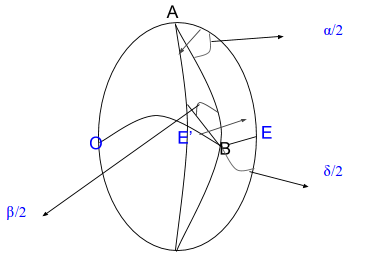
\includegraphics{1.png}
  \caption{Ilustración del problema en el espacio}
  \label{fig:ejemplo}
\end{figure}


y para conseguir las fórmulas que vinculan los triángulos esféricos
utilizamos fórmulas que vinculan a un triángulo plano.\\

\begin{figure}[H]
  \centering
    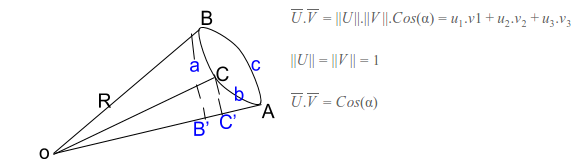
\includegraphics{2.png}
  \caption{Vinculación del triangulo al plano}
  \label{fig:ejemplo}
\end{figure}


\overline{OB}.\overline{OC}=Cos(a)=(\overline{OB'}+\overline{B'B})+(\overline{OC'}+\overline{C'C})=\overline{OB'}.\overline{OC'}+\overline{OB'}.\overline{C'C}+\overline{B'B}.\overline{OC'}+\overline{B'B}.\overline{C'C}=

\(= Cos(c).Cos(b).Cos(0 \circ ) + Cos(c).Sen(b).Cos(90 \circ ) + Sen(c).Cos(b).Cos(90 \circ ) + Sen(c).Sen(b).Cos(A)\)

\(Cos(a) = Cos(c)Cos(b) + Cos(c).Sen(b).Cos(A)\)

\\

\begin{figure}[H]
  \centering
    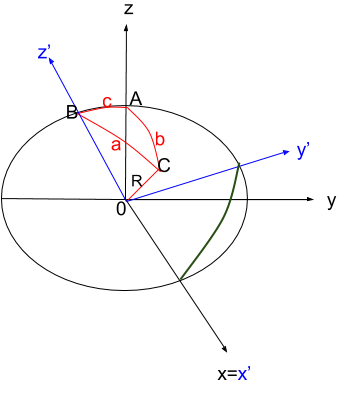
\includegraphics{3.png}
    \caption{Vinculación del triangulo al plano}
  \label{fig:ejemplo}
\end{figure}


\(R = 1\)

\(x' = x\)

\(y' = y.Cos(c) + z.Sen(c)\) 

\(z' = z.Cos(c) - y.Sen(c)\)\(\)

\(x = Sen(b).Sen(A)\) 

\(x' = Sen(a).Sen(B)\)

\(y = Sen(b).Cos(A)\)

\(y' = sen(a)Cos(B)\)

\(z = Cos(b)\) 

\(z' = Cos(a)\)

\(\frac{Sen(A)}{Sen(a)} = \frac{Sen(B)}{Sen(b)} = \frac{Sen(C)}{Sen(c)}\)\\
\\

Los cuaterniones unitarios proporcionan una notación matemática para
representar las orientaciones y las rotaciones de objetos en tres
dimensiones. Comparados con los ángulos de Euler, son más simples de
componer y comparados con las matrices de rotación, son más eficientes y
más estables numéricamente.
\\


\(q = (q_{0},q_{1},q_{2},q_{3})\), \(q_{0} = S\) es un valor y
\((q_{1},q_{2},q_{3}) = \overline{v}\)

\(q=(S,\overline{v}), \overline{q}=(S,\overline{-v})\)

\(q_{0}.q_{1} = (q_{00},q_{01},q_{02},q_{03}).(q_{10},q_{11},q_{12},q_{13}) = (S_{0}.S_{1}, - \overline{v0}.\overline{v1},S0.\overline{v1}+S1.\overline{v0}+\overline{v0} \wedge \overline{v1})\)

\(\text{q.\overline{q}} = q_{0}^{2} + q_{1}^{2} + q_{2}^{2} + q_{3}^{2}\)

\(\text{q.}q^{- 1} = \frac{\overline{q}}{\overline{q}} \Rightarrow q^{- 1} = \frac{\overline{q}}{{||q||}^{2}}\)
y cuando \(q = 1 \Rightarrow q^{- 1} =\overline{q} \)

\(P_{\text{ROT}} = (0,\overline{Vrot}) = q.p.\overline{q}\), con \(p = (0,\overline{v}\) y \(||q|| = 1\)

\section{Desarrollo matemático para encontrar \(\varphi_{p'}\) \emph{y}
\(\lambda_{p'}\)}\\


\emph{Datos:}\\

\(\varphi_{A}\epsilon\ \lbrack 35,55\rbrack\),
\(\lambda_{A}\epsilon\ \lbrack 35,55\rbrack\),\(\varphi_{P}\epsilon\ \lbrack 55,65\rbrack\),
\(\lambda_{P}\epsilon\ \lbrack 55,65\rbrack\),\(\theta\)

\subsection{En esféricas:}\\

\emph{Calculo} \(\widehat{\text{AP}}\)\emph{como:}\\

\(Cos(\widehat{\text{AP}}) = Cos(\varphi_{A}).Cos(\varphi_{P}) + Sen(\varphi_{A})Sen(\varphi_{P})Cos(\widehat{\text{AZP}})\)

Como
\(\widehat{\text{AZP}} = \lambda_{p} - \lambda_{A} \Rightarrow Cos(\widehat{\text{AZP}}) = Cos(\lambda_{p} - \lambda_{A}) \Rightarrow\)

\(\Rightarrow \widehat{\text{AP}} = ARC\ Cos\lbrack Cos(\varphi_{A}).Cos(\varphi_{P}) + Sen(\varphi_{A})Sen(\varphi_{P})Cos((\lambda_{p} - \lambda_{A})\rbrack\)\\

\emph{Calculo} \(\widehat{\text{ZAP}}\)\emph{como:}\\

\(\frac{Sen(\widehat{\text{ZAP}})}{Sen(\varphi_{P})} = \frac{Sen(\widehat{\text{AZP}})}{Sen(\widehat{\text{AP}})}\),
con \(sen(\widehat{\text{AZP}}) = Sen(\lambda_{p} - \lambda_{A})\)y con
dos formas de calcular \(Sen(\widehat{\text{AP}})\):

\begin{itemize}
\item
  \begin{quote}
  \(Sen(\widehat{\text{AP}}) = ARC\ Cos(\widehat{\text{AP}})\)
  \end{quote}
\item
  \begin{quote}
  \(Sen(\widehat{\text{AP}}) = \sqrt{1-Cos^2(\widehat{\text{AP}})}\)
  \end{quote}
\end{itemize}

\(\Rightarrow \widehat{\text{ZAP}} = \ ARC\ Sen\lbrack\frac{\text{Sen}\widehat{\text{AZP}}.Sen(\varphi_{P})}{Sen(\widehat{AP)}}\rbrack\)\\

\emph{Opción 1:}\\

\(ARC\ Sen\ (\widehat{\text{ZAP}}) + \theta = \widehat{ZAP'}\)\\

\emph{Opción 2:}\\

\(Cos(\widehat{ZAP'}) = Cos(\widehat{\text{ZAP}}).Cos(\theta) - Sen(\widehat{\text{ZAP}}).Sen(\theta)\)

\(Sen(\widehat{ZAP'}) = Sen(\widehat{\text{ZAP}}).Cos(\theta) + Cos(\widehat{ZAP)}.Sen(\theta)\)\\

\emph{Calculo} \(\varphi_{p'}\)\emph{como:}\\

\(\varphi_{p'} = \widehat{ZP'} = Cos(\widehat{\text{ZA}}).Cos(\widehat{AP'}) + Sen(\widehat{\text{ZA}}).Sen(\widehat{AP'}).Cos(\widehat{ZAP'})\)

Como
\(\widehat{AP'} = \widehat{\text{AP}} \Rightarrow Sen(\widehat{AP'}) = Sen(\widehat{\text{AP}})\)y
\(Cos(\widehat{AP'}) = Cos(\widehat{\text{AP}})\)

Como
\(\widehat{\text{ZA}} = \varphi_{A} \Rightarrow Cos(\widehat{\text{ZA}}) = Cos(\varphi_{A})\)
y \(Sen(\widehat{\text{ZA}}) = Sen(\varphi_{A})\)

\(\Rightarrow \varphi_{p'} = Cos(\varphi_{A}).Cos(\widehat{\text{AP}}) + Sen(\varphi_{A}).Sen(\widehat{\text{AP}}).Cos(\widehat{ZAP'})\)\\

\emph{Calculo} \(\lambda_{p'}\)\emph{como:}\\

\(\frac{Sen(\widehat{P'ZA)}}{Sen(\widehat{P'A})} = \frac{Sen(\widehat{ZAP'})}{Sen(\widehat{ZP'})}\)

Como
\(\widehat{ZP'} = \varphi_{p'} \Rightarrow Sen(\widehat{ZP'}) = Sen(\varphi_{p'})\)

Como
\(\widehat{P'A} = \widehat{\text{PA}} \Rightarrow Sen(\widehat{P'A}) = Sen(\widehat{\text{PA}})\)

\(\widehat{P'ZA} = ARC\ Sen\ \lbrack\frac{Sen(\widehat{ZAP'}).Sen(\widehat{\text{PA}})}{Sen(\varphi_{p'})}\rbrack\)\\

Finalmente \(\lambda_{p'} = \lambda_{A} - \widehat{P'ZA}\)\\

\subsection{En Cuaterniones:}\\

\(P_{\text{ROT}} = q.p.\overline{q}\)\\

\emph{Donde:}\\

\(q = (Cos(\frac{\theta}{2}),(Sen(\varphi_{A}).Cos(\lambda_{A}),Sen(\varphi_{A}).Sen(\lambda_{A}),Cos(\varphi_{A})).Sen(\frac{\theta}{2}))\)

\(= (Cos(\frac{\theta}{2}), - (Sen(\varphi_{A}).Cos(\lambda_{A}),Sen(\varphi_{A}).Sen(\lambda_{A}),Cos(\varphi_{A})).Sen(\frac{\theta}{2}))\)

\(p = (0,(Sen(\varphi_{p}).Cos(\lambda_{p}),Sen(\varphi_{p}).Sen(\lambda_{p}),Cos(\varphi_{p}))\)

\(P_{\text{ROT}}\)es de la forma \(P_{\text{ROT}} = (0,\overline{Vrot})\) con
\(\overline{Vrot}= (X_{R},Y_{R},Z_{R})\)\\

Finalmente: \(\varphi_{p'} = ARC\ Tan\ \lbrack\frac{\sqrt{(X_{R})^2+(Y_{R})^2}}{Z_{R}}\rbrack\)\\

\(\lambda_{p'} = ARC\ Tan\ \lbrack\frac{Y_{R}}{X_{R}}\rbrack\)
  
\clearpage  
\section{Conclusiones}

A continuación podremos ver reflejado en una tabla y un grafico, los resultados obtenidos mediante la experimentación realizada con el software creado para las mediciones:

\begin{figure}[H]
  \centering
    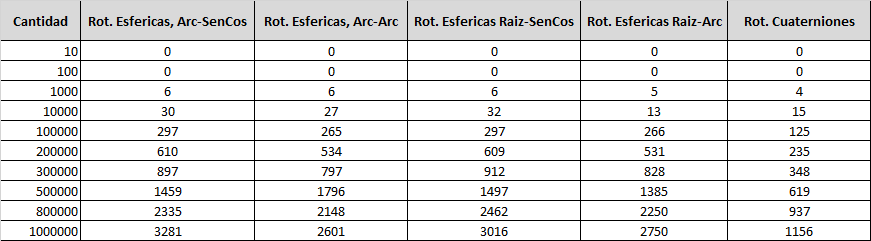
\includegraphics{result.png}
  \caption{Gráfico de barras con resultados}
  \label{fig:ejemplo}
\end{figure}\\

Tiempo en milisegundos\\

\begin{figure}[H]
  \centering
    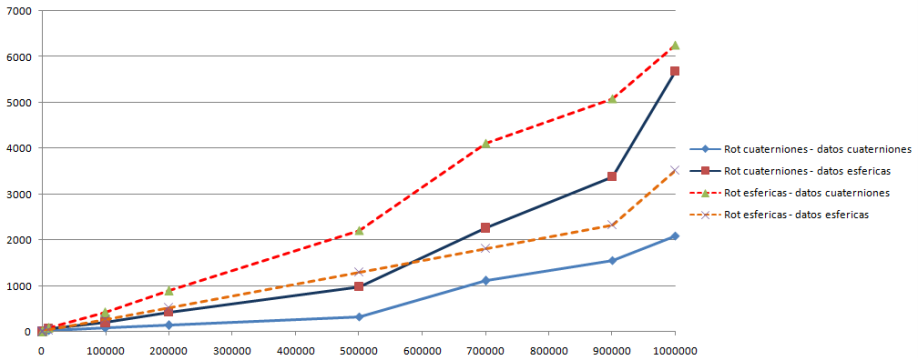
\includegraphics[scale=0.75]{resultgrafico.png}
  \caption{Gráfico extendido}
  \label{fig:ejemplo}
\end{figure}

  
  Con la cantidad de datos empleados para medir la eficiencia de las rotaciones mediante cuaterniones y coordenadas esféricas se puede ver que existe una preeminencia de los mejores tiempos logrados por el método de rotaciones mediante cuaterniones. 
  
  En el mejor de los casos los tiempos logrados con la mayor cantidad de datos de entrada (un millón) indican que es un 57 por ciento menor que con el método de coordenadas esféricas. También se puede ver que, dependiendo del formato de datos de entrada, los valores mejoran considerablemente. Esto indica que los procesos empleados para la conversión de los datos a coordenadas cartesianas juegan un papel muy importante en todo el procedimiento usado para las mediciones de tiempos. Esto se puede ver claramente cuando la cantidad de datos es un millón: los tiempos de procesamiento aumentan un 280 por ciento si los datos de origen están en coordenadas esféricas.Por otro lado si analizamos los resultados obtenidos con coordenadas esféricas podemos ver que la incidencia de la conversión de datos a coordenadas esféricas no es tan grande como con las rotaciones con cuaterniones. 
  
  Para un millón de datos de entrada los tiempos aumentan solo un 75 por ciento.
  Si bien la conversión de los datos de entrada no está relacionada directamente con los métodos de rotación analizados esto puede jugar un rol clave dependiendo de las aplicaciones. Es decir, existen áreas donde el formato del origen de los datos condiciona los métodos a elegir. Por cuestiones de capacidad de los sistemas empleados sólo se pudo llegar a una cantidad de un millón de datos de entrada. 
  
  En principio esto indicaría que el número de datos de entrada puede llegar a jugar un papel destacado en la elección de un método u otro. 
  Pero por otro lado los gráficos sugieren que a la larga, y con mayor cantidad de datos, el método mediante cuaterniones prevalece. Mas a un si consideramos los enormes volúmenes de información empleados hoy en día.
  


  %----------------------------------------------------------------------------------------
  % REFERENCE LIST
  %----------------------------------------------------------------------------------------
\clearpage
  \section{Bibliograf\'ia}

  \begin{thebibliography}{99} 
  
  \bibitem{vision_estereoscopica}
  José Francisco Zelasco , Judith Donayo, Teresa Arcomano: Visión Estereoscópica Búsqueda del Conjunto Mínimo de Puntos Homólogos Para Rotorectificar.
  
  \bibitem{vision_computador}
  Escalera, A., Visión por Computador: Fundamentos y Métodos, Pearson Educación 2001.
  
  \bibitem{repres_cuaternion}
  Del Castillo, G. T. (1999). La representación de rotaciones mediante cuaterniones. Miscelanea Matemtica, 43-50.
  
  \bibitem{teorema_cuatern}
  Guerrero, E., Pacheco, R., & Pérez, E. (2009). El teorema fundamental del álgebra sobre los cuaterniones. Miscelánea Matemática, 50, 77-88.
  
  \bibitem{rotacion_cuatern}
  Serrano, E., Sirne, R. O., & La Mura, G. (2014). Rotaciones, secuencia aeroespacial y cuaterniones. Una revisión de las relaciones fundamentales.

  \end{thebibliography}
  %----------------------------------------------------------------------------------------

\end{document}